\documentclass[twoside]{article}
\usepackage[a4paper]{geometry}
\geometry{verbose,tmargin=2.5cm,bmargin=2cm,lmargin=2cm,rmargin=2cm}
\usepackage{fancyhdr}
\pagestyle{fancy}

% nastavení pisma a češtiny
\usepackage{lmodern}
\usepackage[T1]{fontenc}
\usepackage[utf8]{inputenc}
\usepackage[czech]{babel}

% odkazy
\usepackage{url}

% vícesloupcové tabulky
\usepackage{multirow}
\usepackage{amssymb}
\usepackage{bbold}
\usepackage{amsmath}
\usepackage{commath}

% vnořené popisky obrázků
\usepackage{subcaption}

% automatická konverze EPS 
\usepackage{graphicx} 
\usepackage{epstopdf}
\epstopdfsetup{update}

\graphicspath{{./images}}

% odkazy a záložky
\usepackage[unicode=true, bookmarks=true,bookmarksnumbered=true,
bookmarksopen=false, breaklinks=false,pdfborder={0 0 0},
pdfpagemode=UseNone,backref=false,colorlinks=true] {hyperref}

% Poznámky při překladu
\usepackage{xkeyval}	% Inline todonotes
\usepackage[textsize = footnotesize]{todonotes}
\presetkeys{todonotes}{inline}{}

% Zacni sekci slovem ukol
\renewcommand{\thesection}{Úkol \arabic{section}}
% enumerate zacina s pismenem
\renewcommand{\theenumi}{\alph{enumi}}

% smaz aktualni page layout
\fancyhf{}
% zahlavi
\usepackage{titling}
\fancyhf[HC]{\thetitle}
\fancyhf[HLE,HRO]{\theauthor}
\fancyhf[HRE,HLO]{\today}
 %zapati
\fancyhf[FLE,FRO]{\thepage}

% údaje o autorovi
\title{Domácí úkol 0 - opakování předmětu SAS}

\author{Vojtěch Michal}
\date{\today}

\begin{document}

\maketitle

% ---------------------------------
% ---------------------------------
% název sekce je generován automaticky jako: Úkol X
\section{Ustálená odezva}
\label{sec:ukol1}

\subsection{~}
\label{sec:ukol1:1}
Nalezněte statické zesílení K systému popsaného níže uvedeným přenosem.
\begin{equation}
	G(s) = \frac{-0.2s+5}{(s+3)(s+2)(s+1)}
\end{equation}
Řešení: Statické zesílení je konečná hodnota odezvy na jednotkový skok $w(t)$. Podle věty o konečné hodnotě
\begin{equation}
	\lim_{t \to \infty}w(t) = \lim_{s \to 0}sW(s)
\end{equation}
pro statické zesílení K plyne:
\begin{equation}
	\label{eq:dcgain}
	K = \lim_{t \to \infty}w(t) = \lim_{s \to 0}{\underbrace{sW(s)}_{=G(s)}} = \frac{0+5}{(0+3)(0+2)(0+1)} = \frac{5}{6}.
\end{equation}
Statické zesílení zadaného vnějšího modelu je $K = \frac{5}{6}$.

\subsection{~}
Zjistěte ustálenou hodnotu odezvy na vstup $u (t) = 5$. Své tvrzení odvoďte.

Řešení: Nejdříve je potřeba ověřit, že nějaká ustálená hodnota bude existovat. Zřejmě ano, protože přenosová funkce má všechny póly
v levé polorovině s. Využijeme linearity systému a Laplaceovy transformace. Protože $u(t) = 5\cdot \mathbb{1}(t)$, platí pro výstup $y(t)$:
\begin{equation}
	y(t) = \mathcal{L}^{-1}\{G(s) \cdot \mathcal{L}\{u(t)\}\} = 5~\mathcal{L}^{-1}\{\underbrace{G(s) \cdot \mathcal{L}\{\mathbb{1}(t)\}}_{= \frac{1}{s}G(s)=W(s)}\}
	= 5 w(t) \longrightarrow_{t \to \infty} 5 K.
\end{equation}
Se znalostí statického zesílení podle \eqref{eq:dcgain} je vidět, že se výstup ustálí na hodnotě $y(t)=\frac{25}{6}$.


\subsection{~}
\label{sec:ukol1:3}
Jaká bude ustálená hodnota odezvy na Dirakův impulz? \\
Řešení: Odezvy na jednotkový skok $w(t)$ a na Diracův impuls $h(t)$ spojuje vztah $w(t) = \int h(t)$. Z \ref{sec:ukol1:1} již víme, že $w(t)$ se ustálí
na konstantní hodnotě $K$, její derivace $h(t)$ tedy po ustálení musí být nulová. Pro ustálenou hodnotu impulsové odezvy tedy platí $\lim_{t \to \infty} h(t) = 0$.

% ---------------------------------
\section{Laplaceova transformace}
\label{sec:ukol2}
\subsection{~}
Pomocí Laplaceovy transformace vyřešte následující soustavu diferenciálních rovnic
\begin{equation*}
	\begin{split}
		\dot{x_1} &= - 6x_1 (t) + 26x_2 (t), \\
		\dot{x_2} &= - 0.5 x_1(t),
	\end{split}
\end{equation*}
za počátečních podmínek
\begin{equation*}
	\vec{x}_0 = \begin{bmatrix}
		2 \\
		0
	  \end{bmatrix}.
\end{equation*} \\
Řešení: Převeďme soustavu do maticového tvaru
\begin{equation*}
	\dot{\vec{x}}(t) = \underbrace{\begin{bmatrix}
		-6 & 26 \\
		-0.5 & 0
	\end{bmatrix}}_{A} \vec{x}(t)
\end{equation*}
a transformujme Laplaceovou transformací. Nechť $\mathcal{L}\{\vec{t}(t)\} = X(s)$, poté
\begin{equation*}
	s\vec{X}(s) - \vec{x_0} = A\vec{X}(s) \Rightarrow \vec{X}(s) = (sI-A)^{-1}\vec{x_0}.
\end{equation*}
Po dosazení zadaných hodnot do rovnice získám
\begin{equation*}
	\vec{X}(s) = \underbrace{\begin{bmatrix}
		s + 6 & -26 \\
		0.5 & s
	\end{bmatrix}^{-1}}_{=(sI - A)} \begin{bmatrix}
		2 \\
		0
	\end{bmatrix} = \underbrace{\frac{1}{s(s+6) + 13}}_{=\text{det}^{-1}(sI - A)} \underbrace{\begin{bmatrix}
		s & 26 \\
		-0.5 & s + 6
	\end{bmatrix}}_{\text{adj}(sI - A)} \begin{bmatrix}
		2 \\
		0
	\end{bmatrix} = \frac{1}{s^2 + 6s + 13} \begin{bmatrix}
		2s \\
		-1
	\end{bmatrix}.
\end{equation*}
Pro obrazy funkcí $x_1(t)$, $x_2(t)$ po složkách platí
\begin{equation*}
	\begin{split}
		x_1(s) &= \frac{2s}{s^2 + 6s + 13} \\
		x_2(s) &= \frac{-1}{s^2 + 6s + 13}
	\end{split}
\end{equation*}
a obě rovnice invertujeme. Jmenovatel má kořeny $s_{1,2} = -3 \pm 2i$, označme $\sigma = -3$, $\omega = 2$. Očekávám, že řešení bude složeno 
z kvazipolynomů s $\text{exp}(\sigma t)$, $\text{sin}(\omega t)$ a $\text{cos}(\omega t)$.
\begin{equation*}
	\begin{split}
		x_1(t) &= \mathcal{L}^{-1}\{\frac{2s}{(s+3)^2 + 4}\} = \mathcal{L}^{-1}\{\frac{2(s - \sigma)}{(s-\sigma)^2 + \omega^2}\} + \mathcal{L}^{-1}\{\frac{2\sigma}{(s-\sigma)^2 + \omega^2}\} = 
		2 e^{\sigma t} \text{cos}(\omega t) + 2 \frac{\sigma}{\omega} e^{\sigma t} \text{sin}(\omega t),\\
		x_2(t) &= \mathcal{L}^{-1}\{\frac{-1}{(s+3)^2 + 4}\} = \mathcal{L}^{-1}\{\frac{-0.5 \omega}{(s-\sigma)^2 + \omega^2}\} = -\frac{1}{2} e^{\sigma t} \text{sin}(\omega t).
	\end{split}
\end{equation*}
Po vyčíslení obdržíme
\begin{equation*}
	\begin{split}
		x_1(t) &= e^{-3t}(2\text{cos}(2t) -3 \text{sin}(2t)), \\
		x_2(t) &= -0.5 e^{-3t}\text{sin}(2t).
	\end{split}
\end{equation*}

\subsection{~}
\begin{figure}[htb]
	\includegraphics{solution22.eps}
	\label{fig:reseni22}
\end{figure}
Vykreslete průběhy nalezených funkcí v Matlabu. Nezapomeňte na popisky os, titulek, legendu a přehlednost - tedy vše,
co by se v mělo u Vašich grafů v budoucnu vždy objevit. \\
Řešení je vykresleno na \ref{fig:reseni22}.

\section{Linearizace}
\label{sec:ukol3}
Je zadaný systém
\begin{equation}
	\begin{split}
		\dot{x_1} &= x_2 \\
		\dot{x_2} &= -2 \text{sin}(x_1) - 0.1x_2 +u \\
		y &= x_1
	\end{split}
\end{equation}

\subsection{~}
Nalezněte rovnovážný pracovní bod systému $P = \begin{bmatrix} x_{1p}, x_{2p}, y_p \end{bmatrix}$ pro $u_p (t) = 2$.

\subsection{~}
Linearizujte systém v nalezeném pracovním bodě $P$.

\subsection{~}
Namodelujte v Simulinku nelineární systém současně s linearizovaným. Porovnejte odezvy obou systémů
na skok $u(t) = 1$ a $u(t) = 2.001$. Průběhy nelineárního a linearizovaného systému vykreslete do jednoho
obrázku pomocí Matlabu.

\section{Asymptotické frekvenční charakteristiky}
\label{sec:ukol4}

\subsection{~}
Pro následující systém nakreslete asymptotickou frekvenční charakteristiku.
\begin{equation}
	G_1(s) = \frac{s-1}{(s+10)(s-10)(s+80)}
\end{equation}
Řešení: Přenos nejprve upravím do podoby vhodné pro vyšetřování frekvenční charakteristiky.
\begin{equation*}
	G_1(s) = \frac{s-1}{8000(\frac{s}{10}+1)(\frac{s}{10}-1)(\frac{s}{80}+1)} = \frac{1}{8000} \frac{\frac{s}{\omega_1}-1}{(\frac{s}{\omega_2}+1)(\frac{s}{\omega_2}-1)(\frac{s}{\omega_3}+1)}
\end{equation*}
Významné body tak jsou nula na frekvenci $\omega_1 = 1 \text{rad.s}^{-1}$, dvojnásobný pól na frekvenci $\omega_2 = 10 \text{rad.s}^{-1}$ a pól na $\omega_3 = 80 \text{rad.s}^{-1}$.
Výsledná frekvenční i amplitudová charakteristika se bude skládat z příspěvků od dílčích kořenových činitelů v čitateli i jmenovateli.
\todo{finish}

\subsection{~}
\begin{figure}
	\includegraphics{zadani4-2.png}
	\label{fig:zadani4}
\end{figure}
Pro asymptotickou frekvenční charakteristiku na obrázku \ref{fig:zadani4} sestavte rovnici odpovídajícího systému
s nejnižším možným počtem pólů. \\
Řešení: Významné body charakteristiky jsou
\begin{itemize}
	\item jednoduchý pól na $\omega_1 = 10^{-3}~\text{rad.s}^{-1}$,
	\item jednoduchá nula na $\omega_2 = 10^{-1}~\text{rad.s}^{-1}$,
	\item jednoduchá nula na $\omega_3 = 10^1~\text{rad.s}^{-1}$,
	\item jednoduchý pól na $\omega_4 = 10^3~\text{rad.s}^{-1}$,
\end{itemize}
dále pro DC signál ($s = 0$) je zesílení 0dB, takže přenosová funkce nebude obsahovat skalární činitele.
Na základě amplitudové charakteristiky očekávám přenosovou funkci tvaru
\begin{equation*}
	H(s) = \pm \frac{(\frac{s}{\omega_2}\pm 1)(\frac{s}{\omega_3} \pm 1)}{(\frac{s}{\omega_1}\pm 1)(\frac{s}{\omega_4} \pm 1)}.
\end{equation*}
O rozložení plus a mínus rozhodneme na základě fázové charakteristiky.
\begin{equation*}
	H(s) = - \frac{(\frac{s}{\omega_2} + 1)(\frac{s}{\omega_3} + 1)}{(\frac{s}{\omega_1} + 1)(\frac{s}{\omega_4} + 1)}.
\end{equation*}
\todo{finish}
\section{ Převod do přenosového popisu}
\label{sec:ukol5}
Převeďte následující systém do přenosového popisu. Napište postup, kterým jste k výsledku dospěli, a vybrané mezivýsledky.

\begin{math}
	\dot{\vec{x}} = \begin{bmatrix}
		-4 & 2 & 0 & 0 \\
		-6 & 4 & 0 & 0 \\
		-3 & 3 & 2 & -2 \\
		-9 & 9 & 2 & -3
	\end{bmatrix} \vec{x} + \begin{bmatrix}
		1 \\
		0.5 \\
	0 \\
	-1
\end{bmatrix} u ~~~~~~~~~~~
y = \begin{bmatrix}
	4 & 0 & 0 & 0
\end{bmatrix} \vec{x}
\end{math} \\
Řešení: Odvoďme maticový vzoreček pomocí stavové a výstupní rovnice a Laplaceovy transformace:
\begin{equation*}
	\begin{split}
		sX(s) &= AX(s) + B U(s) \\
		(sI - A) X(s) &= BU(s) \\
		X(s) &= (sI - A)^{-1} B U(s) \\
		Y(s) &= C \underbrace{(sI - A)^{-1} B U(s)}_{=X(s)}.
	\end{split}
\end{equation*}
Odvození je zjednodušené o to, že matice D je nulová. Přenost systému pomocí matic A, B, C poté má tvar
\begin{equation}
	H(s) = \frac{Y(s)}{U(s)} = C(sI-A)^{-1} B.
\end{equation}
Pro zadané matice vrátí Matlab numerické řešení
\begin{equation*}
	H(s) = \frac{4 s^3 - 12 s^2 - 16s + 48}{s^4 - 8 s^2 + 16}.
\end{equation*}
Dává toto řešení smysl? Ve jmenovateli bychom měli mít výraz $ \det{sI - A}$, což je skutečně polynom čtvrtého
řádu v s. Dále je $D = 0$, takže by přenos měl být striktně ryzí a to je též splněno. Podobné řešení bych očekával.

\section{Stabilita}
\label{sec:ukol6}
Rozhodněte o stabilitě systému. Výsledek zdůvodněte.

\begin{math}
	\dot{\vec{x}} = \begin{bmatrix}
		1 & 0 & 0 \\
		2 & -2 & -2 \\
		1 & 2 & 0
	\end{bmatrix} \vec{x} + \begin{bmatrix}
		1 \\
		-1 \\
		1
\end{bmatrix} u ~~~~~~~~~~~
y = \begin{bmatrix}
	1 & 0 & -1
\end{bmatrix} \vec{x}
\end{math} \\
Řešení: Pro rozhodnutí o stabilitě ze stavového popisu lze vyšetřit znaménko vlastních čísel matice systému A.
Stabilní bude systém tehdy, když vlastní čísla budou mít zápornou reálnou část. Toto platí proto, že při převodu
stavového popisu na vnější se do jmenovatele přenosu dostane výraz $\det(sI - A)$. To je polynom v s, jeho kořeny
jsou vlastní čísla matice A, která se tak stávají póly přenosové funkce (předpokládejme, že se v přenosové funkci nic nepokrátí).

Pro zadanou matici mají vlastní čísla hodnotu $1$ a $ -1 \pm 1.73 i$. Kritérium stability tedy není splněno a systém \textbf{není stabilní} 


\section{Diskretizace}
\label{sec:ukol7}
Následující systém převeďte do diskrétního popisu, můžete využít např. metodu \textit{zero order hold}.
\begin{equation}
	G(s) = \frac{s-3}{(s+1)(s+7)}
\end{equation}
K diskretizaci můžete využít Matlab. Následně v Simulinku odsimulujte odezvy diskrétního a spojitého systému
pro dvě různé periody vzorkování - pro jednu vhodně zvolenou (dostatečně krátkou) a jednu nevhodně zvolenou.
Do jednoho grafu vykreslete výstup spojitého systému a výstup diskretizovaného systému s vhodně zvolenou
periodou vzorkování. (1b.) Druhý graf obdobně pro nevhodnou periodu vzorkování. (2b.) Jako vstup zvolte
libovolný periodický signál, např. sinus, pila, atd. Nezapomeňte na to, jak mají vypadat výsledné grafy

\section{Vlastnosti přenosů}
\label{sec:ukol8}
Rozhodněte u každého z následujích přenosů, zdali jím popsaný systém je: stabilní/nestabilní, statický/astatický, kmitavý/nekmitavý.
\begin{equation*}
	\begin{split}
		G_1(s) &= -\frac{s-12}{(s+1)(5s+2)(s+3)} = -\frac{1}{5}~\frac{s-12}{(s+1)(s+0.4)(s+3)} \\
		G_2(s) &= \frac{1}{s^2 + 0.5s - 1} = \frac{1}{(s-0.7808)(s+1.2808)} \\
		G_3(s) &= \frac{1}{s^2} \\
		G_4(s) &= \frac{s+2}{s^2-2} = \frac{s+2}{(s-\sqrt{2})(s+\sqrt{2})}
	\end{split}
\end{equation*}

Vlastnosti budu vyčítat zejména z pólů přenosových funkcí, proto jsme rovnou rozložili polynomy na kořenové činitele.

\begin{itemize}
	\item \textbf{Stabilita}: Stabilní systém má reálnou složku všech pólů zápornou. Toto kritérium splňuje pouze systém s přenosem $G_1(s)$,
	ostatní mají alespoň jeden pól na imaginární ose nebo vlevo od ní.
	\item \textbf{Astatismus}: Astatický systém máintegrační charakter, jeho chování je závislé na přechodím stavu. Přenos astatického 
	systému obsahuje alespoň jeden pól v počátku. Astatický je jen systém s přenosem $G_3(s)$, ostatní jsou statické.
	\item \textbf{Kmitání}: Systém s komplexně sdruženými póly bude kmitat, protože se do jeho impulsové charakteristiky promítnou goniometrické funkce
	(reálná a imaginární složka komplexní exponeniciály). Všechny zadané systémy ale mají póly reálné a tudíž kmitání nemůže nastat.
\end{itemize}






















\section{Spojování dynamických systémů}
\label{sec:ukol9}
Jsou dány dva systémy
\begin{equation*}
	G_1(s) = \frac{s-1}{s+1}, G_2(s) = \frac{1}{s}
\end{equation*}
odvoďte výsledný přenost $H(s)$ pro jejich různá zapojení.
\begin{figure}[htbp]
	\centering
	\includegraphics[width=.4\textwidth]{zadani9-3.png}
	\caption{Zapojení pro úlohu 9.3}
	\label{fig:zadani9-3}
\end{figure}
\begin{figure}[htbp]
	\centering
	\includegraphics[width=.4\textwidth]{zadani9-4.png}
	\caption{Zapojení pro úlohu 9.4}
	\label{fig:zadani9-4}
\end{figure}
\subsection{Paralelní zapojení} 
Řešení: Paralelní zapojení systémů vede na prostý součet jejich přenosů. Proto je celkový přenos zapojení roven
\begin{equation*}
	H(s) = G_1(s) + G_2(s) = \frac{s-1}{s+1} + \frac{1}{s} = \frac{s(s-1) + (s+1)}{s(s+1)} = \frac{s^2 + 1}{s (s+1)}
\end{equation*}
\subsection{Kaskádní spojení}
\label{sec:ukol9:2}
Řešení: Kaskádní spojení vede na konvoluci v časové oblasti a násobení přenosů v oblasti obrazové. Proto je celkový přenos zapojení roven
\begin{equation*}
	H(s) = G_1(s) \cdot G_2(s) = \frac{s-1}{s(s+1)}
\end{equation*}
\subsection{Záporná zpětná vazba } 
\label{sec:ukol9:3}
Zpětnovazební spojení se zápornou zpětnou vazbou, kde přenosy G1 a G2 jsou v přímé vazbě (viz obr \ref{fig:zadani9-3}) \\
Řešení: Označme přenos kaskádního zapojení $G_1(s)$, $G_2(s)$ jako $G(s) = G_1(s)G_2(s) = \frac{s-1}{s(s+1)}$ (podle \ref{sec:ukol9:2}).
Tím se systém zjednodušil na jediný systém zapojený v dopředné cestě zpětnovazební smyčky. Označíme-li $x(s)$ signál za sčítačkou, poté platí
\begin{equation*}
	y(s) = G(s) \cdot x(s) = G(s) \cdot (r(s) - y(s)) \Rightarrow y(s) (1 + G(s)) = G(s) \cdot r(s).
\end{equation*}
Celkový přenos systému je
\begin{equation*}
	H(s) = \frac{y(s)}{r(s)} = \frac{G(s)}{1 + G(s)} = \frac{s^3 - s}{s^4 + 3s^3 + s^2 - s}.
\end{equation*}
\subsection{Záporná zpětná vazba } 
Zpětnovazební spojení se zápornou zpětnou vazbou s G1 v přímé vazbě a G2 ve zpětné vazbě (viz obr \ref{fig:zadani9-4}) \\
Řešení: Podobně jako \ref{sec:ukol9:3} popíši systém rovnicemi. Označme $x(s)$ signál na výstupu sčítačky. Podle schématu platí:
\begin{equation*}
	y(s) = G_1(s) \cdot x(s) = G_1(s) \cdot (r(s) - G_2(s) \cdot y(s)) \Rightarrow y(s) (1 + G_1(s)G_2(s)) = G_1(s) \cdot r(s).
\end{equation*}
Celkový přenos systému je
\begin{equation*}
	H(s) = \frac{y(s)}{r(s)} = \frac{G_1(s)}{1 + G_1(s)G_2(s)} = \frac{s^3 - s}{s^3 + 3s^2 +s - 1}.
\end{equation*}
\section{Diskrétní systém}
\label{sec:ukol10}
Je zadán diskrétní systém
\begin{equation}
	\label{eq:diferencni}
	3y(k) - y(k-1) + 0.5 y(k-2) = u(k-1)-u(k-2)
\end{equation}

\subsection{~}
Vyjádřete přenos systému. \\
Řešení: Použiji Z-transformaci diferenční rovnice popisující systém. Nechť $Y(z) = \mathcal{Z}\{y(k)\}$ a $U(z) = \mathcal{Z}\{u(k)\}$, poté \eqref{eq:diferencni} upravíme na
\begin{equation}
	\begin{split}
		3Y(z) - z^{-1} Y(z) + 0.5 z^{-2} Y(z) &= z^{-1}U(z) - z^{-2}U(z) \\
		Y(z) (3- z^{-1} + 0.5 z^{-2}) &= U(z) (z^{-1} - z^{-2}) \\
		H(z) = \frac{Y(z)}{U(z)} &= \frac{z^{-1} - z^{-2}}{3-z^{-1}+ 0.5z^{-2}}, \text{rozšiřme členem $z^2$} \\
		H(z) &= \frac{z - 1}{3z^2-z+ 0.5}.
	\end{split}
\end{equation}

\subsection{~}
Rozhodněte o stabilitě systému. Rozhodnutí zdůvodněte.
Řešení: Přenosová funkce má dva komplexně sdružené póly $ z_{1,2} = 0.1667 \pm 0.3727i$. Aby byl stabilní, musí ležet póly uvnitř jednotkové kružnice v z-rovině.
Tento požadavek je zde zřejmě splněn, protože $\vert z_{1,2} \vert < 1 $ a systém je tedy stabiltní.
\subsection{~}
Nakreslete simulinkové schéma realizace tohoto přenosu pro vstup u a výstup y a vykreslete jeho odezvu
na jednotkový skok pro vzorkovací periodu h = 1
\todo{Do this}


\section{ Skokové (přechodové) a impulzní charakteristiky}
\label{sec:ukol11}
Na obrázku \ref{fig:charakteristiky} jsou zobrazeny tři impulzní a tři přechodové charakteristiky pro tři různé systémy

\subsection{~}
Přiřaďte správně skokové charakteristiky impulzním charakteristikám tak, aby odpovídaly stejnému systému. \\
Řešení: S ohledem na \ref{sec:ukol11:2} lze k sobě přiřadit odezvy podle tabulky \ref{tab:odezvy}.
\begin{table}[htbp]
	\label{tab:odezvy}
	\centering
	\begin{tabular}{c|c|c}
		$h(t)$ & $w(t)$ & poznámka \\
		\hline
		c & e & integrál konstantní $h(t) \neq 0 $ roste lineárně a diverguje \\
		b & d & $h(t)$ i $w(t)$ exponeniciální průběh \\
		a & f & $h(t)$ kmitá, kmihy musíme najít i na $w(t)$
	\end{tabular}
	\caption{Přiřazení odezvy na Diracův impuls a na jednotkový skok}
\end{table} 

\subsection{~}
\label{sec:ukol11:2}
Jaký obecně mezi sebou mají impulzní charakteristika $h(t)$ a skoková charakteristika $w(t)$ vztah? \\
Řešení (viz \ref{sec:ukol1:3}): Protože spojitý lineární systém zachovává vztahy jako integrál, derivace a lineární kombinace,
je vztah $h(t)$ a $w(t)$ stejný jako vztah signálů $\delta(t)$ a $\mathbb{1}$(t). Platí
\begin{equation*}
	h(t) = \frac{\dif}{\dif t} w(t) ~~ a ~~~~~~~~~ w(t) = \int_0^{t} h(\tau) \dif \tau.
\end{equation*}


\begin{figure}[htbp]
    \centering % <-- added
\begin{subfigure}{0.25\textwidth}
  \includegraphics[width=\linewidth]{zadani11-a}
  \caption{}
  \label{fig:charakteristiky:a}
\end{subfigure}\hfil % <-- added
\begin{subfigure}{0.25\textwidth}
	\includegraphics[width=\linewidth]{zadani11-b}
	\caption{}
	\label{fig:charakteristiky:b}
\end{subfigure}\hfil % <-- added
\begin{subfigure}{0.25\textwidth}
	\includegraphics[width=\linewidth]{zadani11-c}
	\caption{}
  \label{fig:charakteristiky:c}
\end{subfigure}

\medskip
\begin{subfigure}{0.25\textwidth}
  \includegraphics[width=\linewidth]{zadani11-d}
  \caption{}
  \label{fig:charakteristiky:d}
\end{subfigure}\hfil % <-- added
\begin{subfigure}{0.25\textwidth}
	\includegraphics[width=\linewidth]{zadani11-e}
	\caption{}
	\label{fig:charakteristiky:e}
\end{subfigure}\hfil % <-- added
\begin{subfigure}{0.25\textwidth}
	\includegraphics[width=\linewidth]{zadani11-f}
  \label{fig:charakteristiky:f}
  \caption{}
\end{subfigure}
\caption{Charakteristiky k identifikaci}
\label{fig:charakteristiky}
\end{figure}


\section{Frekvenční charakteristiky}
\label{sec:ukol12}
Na obrázku \ref{fig:frekchar} jsou zobrazeny Bodeho frekvenční charakteristiky a Nyquistovy frekvenční charakteristiky tří systémů.
\subsection{~}
Přiřaďte k sobě frekvenční charakteristiky odpovidající stejnému systému. \\
Řešení: Při přiřazení charakteristik si musím vystačit s obecným trendem fáze a amplitudy, protože z Nyquistovy char. nelze odečíst přesná frekvence.
Amplitudy v této úloze nebyly příliš nápomocné, všechny charakteristiky lze určit pohledem na fáze. Jedna dvojice má fáze konstantní,
druhá dvojice mění fázi na celém spektru jen o 90° a poslední o 270°.
Charakteristiky lze přiřadit podle tabulky \ref{tab:charakteristiky}.
\begin{table}[htbp]
	\label{tab:charakteristiky}
	\centering
	\begin{tabular}{c|c|c}
		Bode & Nyquist & poznámka \\
		\hline
		c & e & jediná možnost s konstantní fází, amplitudy omezeny shora \\
		a & f & pro $\omega \rightarrow 0$ je fáze 0, celkem změna fáze o 90° \\
		b & d & celkem změna fáze o 270°
	\end{tabular}
	\caption{Přiřazení odpovídajícíh si frekvenčních charakteristik}
\end{table}
\subsection{~}
U frekvenční charakteristiky na obrázku \ref{fig:frekchar:f} najděte pro fázi -45° zesílení systému (v dB). \\
Řešení: Komplexní čísla $z$ s fází -45° leží na přímce s předpisem $ \Re(z) = - \Im(z)$. Jejím průsečíkem s danou Nyquistovou charakteristikkou
je bod $z_0 = 0.5 - 0.5i$. Zesílení systému v daném bodě charakteristiky je 
\begin{equation}
	\abs{z} = \sqrt{\frac{2}{4}} = \frac{1}{\sqrt{2}},
\end{equation}
což v logaritmických souřadnicích odpovídá zesílení $20 \log{\frac{1}{\sqrt{2}}} = -3$ dB.


\begin{figure}[htbp]
    \centering % <-- added
\begin{subfigure}{0.25\textwidth}
  \includegraphics[width=\linewidth]{zadani12-a}
  \caption{}
  \label{fig:frekchar:a}
\end{subfigure}\hfil % <-- added
\begin{subfigure}{0.25\textwidth}
	\includegraphics[width=\linewidth]{zadani12-b}
	\caption{}
	\label{fig:frekchar:b}
\end{subfigure}\hfil % <-- added
\begin{subfigure}{0.25\textwidth}
	\includegraphics[width=\linewidth]{zadani12-c}
  \caption{}
  \label{fig:frekchar:c}
\end{subfigure}

\medskip
\begin{subfigure}{0.25\textwidth}
  \includegraphics[width=\linewidth]{zadani12-d}
  \caption{}
  \label{fig:frekchar:d}
\end{subfigure}\hfil % <-- added
\begin{subfigure}{0.25\textwidth}
	\includegraphics[width=\linewidth]{zadani12-e}
	\caption{}
	\label{fig:frekchar:e}
\end{subfigure}\hfil % <-- added
\begin{subfigure}{0.25\textwidth}
	\includegraphics[width=\linewidth]{zadani12-f}
  \caption{}
  \label{fig:frekchar:f}
\end{subfigure}
\caption{Frekvenční charakteristiky ke spojení}
\label{fig:frekchar}
\end{figure}




% ---------------------------------
% ---------------------------------
% Literatura
\begin{thebibliography}{9}

% vzorová citace
\bibitem{lamport94}
  Leslie Lamport,
  \emph{\LaTeX: A Document Preparation System}.
  Addison Wesley, Massachusetts,
  2nd Edition,
  1994.

\bibitem{Wiki}
	\LaTeX tutorials, \url{http://en.wikibooks.org/wiki/LaTeX/}

\bibitem{ARI11}
	Studenti předmětu ARI 2011, \emph{ARI song (videoklip)} \url{http://www.youtube.com/watch?v=5gDfQK7dD7c}
\end{thebibliography}












\end{document}

